\documentclass[9pt,aspectratio=169]{beamer}

% ===================== PACKAGES =====================
\usepackage[utf8]{inputenc}
\usepackage[T1]{fontenc}
\usepackage{lmodern}
\usepackage{helvet}
\renewcommand{\familydefault}{\sfdefault}
\usepackage{tikz}
\usetikzlibrary{arrows.meta,positioning,shapes,fit,backgrounds,decorations.pathreplacing}
\usepackage{forest}
\usepackage{pgfplots}
\pgfplotsset{compat=1.17}
\usepackage{algorithm}
\usepackage{algpseudocode}
\usepackage{booktabs}
\usepackage{array}
\usepackage{amsmath,amssymb}
\usepackage{ragged2e}

% ===================== COLOR PALETTE =====================
\definecolor{darkblue}{HTML}{102A43}
\definecolor{midblue}{HTML}{28517A}
\definecolor{teal}{HTML}{0F9B8E}
\definecolor{tealLight}{HTML}{DFF5F2}
\definecolor{grey}{HTML}{627D98}
\definecolor{lightgrey}{HTML}{F0F4F8}
\definecolor{paleGrey}{HTML}{D9E2EC}
\definecolor{warnRed}{HTML}{C2452D}

% ===================== MINIMAL MODERN THEME =====================
\usetheme{default}
\setbeamertemplate{navigation symbols}{}
\setbeamercolor{background canvas}{bg=white}
\setbeamercolor{normal text}{fg=darkblue}
\setbeamercolor{structure}{fg=teal}
\setbeamercolor{title}{fg=darkblue}
\setbeamercolor{author}{fg=grey}
\setbeamercolor{itemize item}{fg=teal}
\setbeamercolor{itemize subitem}{fg=grey}
\setbeamercolor{block title}{bg=darkblue,fg=white}
\setbeamercolor{block body}{bg=lightgrey,fg=darkblue}
\setbeamerfont{frametitle}{size=\Large,series=\bfseries}
\setbeamerfont{framesubtitle}{size=\normalsize,series=\mdseries}
\setbeamertemplate{itemize items}[circle]
\setbeamertemplate{enumerate items}[default]

\setbeamertemplate{frametitle}{
  \vspace{2mm}
  \begin{beamercolorbox}[wd=\paperwidth,leftskip=8mm,rightskip=8mm]{frametitle}
    \usebeamerfont{frametitle}\insertframetitle\par
    {\small\color{grey}\insertframesubtitle}
  \end{beamercolorbox}
  \vspace{-2mm}
  
\begin{tikzpicture}\draw[teal,line width=1.4pt] (0,0) -- (\paperwidth,0);\end{tikzpicture}
}

\setbeamertemplate{footline}{
  \begin{beamercolorbox}[wd=\paperwidth,ht=3.2mm,dp=1mm,leftskip=4mm,rightskip=4mm]{footline}
    {\tiny\color{grey}Sorting Algorithms: Merge, Quick \& Heap Sort \hfill Group 7 -- DSMA 123 \hfill \insertframenumber/\inserttotalframenumber}
  \end{beamercolorbox}
}

% ---- helper commands ----
\newcommand{\sectionsep}[1]{%
\begin{frame}[plain]
  \begin{tikzpicture}[remember picture,overlay]
    \fill[darkblue] (current page.south west) rectangle (current page.north east);
    \node[white,font=\Huge\bfseries,align=center] at (current page.center) {#1};
  \end{tikzpicture}
\end{frame}}

\title{\textbf{Sorting Algorithms}}
\subtitle{Merge Sort \(\cdot\) Quick Sort \(\cdot\) Heap Sort}
\author{Anush Kayastha \(\cdot\) Garina Maharjan \(\cdot\) Rastiryata Nepal \(\cdot\) Swopnim Ghimire}
\institute{Group 7 \\ DSMA-123: Data Structures \\ Department of Mathematics, School of Science \\ Kathmandu University \\[1mm] \textit{Submitted to Dr. Ram Chandra Dhungana}}
\date{14 July 2026}

\begin{document}

% ============================================================
\begin{frame}[plain]
\begin{tikzpicture}[remember picture,overlay]
  \fill[darkblue] (current page.south west) rectangle (current page.north east);
  \fill[teal] (current page.south west) rectangle ++(\paperwidth,0.6);
  \node[align=center,white] at (current page.center) {
    \begin{minipage}{0.85\paperwidth}
      \centering
      {\Huge\bfseries Sorting Algorithms}\\[3mm]
      {\Large Merge Sort \(\cdot\) Quick Sort \(\cdot\) Heap Sort}\\[8mm]
      {\large Divide, Conquer, and Heapify: Three Paths to \(\Theta(n\log n)\)}\\[10mm]
      {\normalsize Anush Kayastha \(\cdot\) Garina Maharjan \(\cdot\) Rastiryata Nepal \(\cdot\) Swopnim Ghimire}\\[2mm]
      {\small Group 7 \(\cdot\) DSMA-123: Data Structures \(\cdot\) Kathmandu University}\\[2mm]
      {\small Submitted to Dr.\ Ram Chandra Dhungana \(\cdot\) 14 July 2026}
    \end{minipage}
  };
  \node[anchor=south east,white,opacity=0.9] at ([xshift=-6mm,yshift=6mm]current page.south east)
   {\begin{tikzpicture}
      \foreach \x/\v in {0/5,1/2,2/8,3/1,4/9,5/3}{
        \draw[fill=teal,draw=white] (\x*0.5,0) rectangle ++(0.4,\v*0.18+0.2);
      }
    \end{tikzpicture}};
\end{tikzpicture}
\end{frame}

% ============================================================
\begin{frame}{Agenda}
\begin{columns}[T]
\begin{column}{0.5\textwidth}
\begin{enumerate}
  \setlength\itemsep{4mm}
  \item Why Sorting Matters
  \item Introduction to Sorting
  \item Algorithms Overview
  \item Merge Sort
  \item Quick Sort
\end{enumerate}
\end{column}
\begin{column}{0.5\textwidth}
\begin{enumerate}
  \setlength\itemsep{4mm}
  \setcounter{enumi}{5}
  \item Heap Sort
  \item Mathematical Analysis
  \item Complexity Comparison
  \item When to Use Which
  \item Conclusion
\end{enumerate}
\end{column}
\end{columns}
\end{frame}

% ============================================================
\begin{frame}{Why Sorting Matters}{A hidden step behind almost every system}
\begin{center}
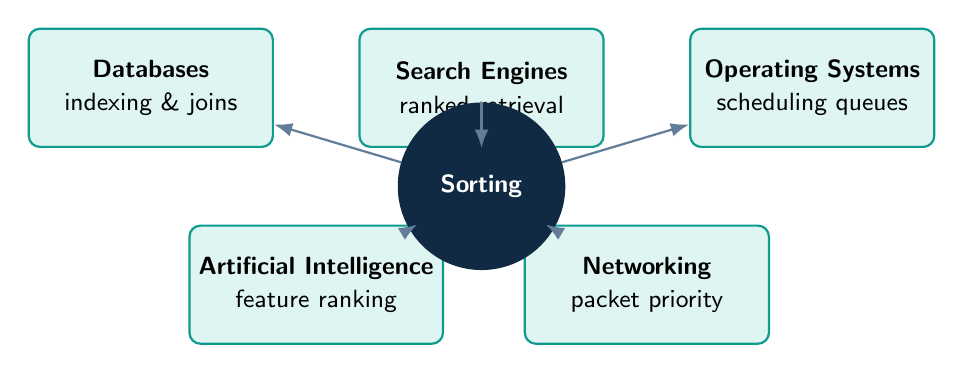
\begin{tikzpicture}[every node/.style={font=\small},box/.style={rectangle,rounded corners,draw=teal,fill=tealLight,minimum width=3.1cm,minimum height=1.5cm,align=center,thick}]
  \node[box] (db) at (0,2.2) {\textbf{Databases}\\[1pt]indexing \& joins};
  \node[box] (se) at (4.2,2.2) {\textbf{Search Engines}\\[1pt]ranked retrieval};
  \node[box] (os) at (8.4,2.2) {\textbf{Operating Systems}\\[1pt]scheduling queues};
  \node[box] (ai) at (2.1,-0.3) {\textbf{Artificial Intelligence}\\[1pt]feature ranking};
  \node[box] (net) at (6.3,-0.3) {\textbf{Networking}\\[1pt]packet priority};
  \node[draw=darkblue,fill=darkblue,text=white,circle,minimum size=2.1cm,thick] (core) at (4.2,0.95) {\textbf{Sorting}};
  \foreach \n in {db,se,os,ai,net}{\draw[-{Latex},grey,thick] (core) -- (\n);}
\end{tikzpicture}
\end{center}
\vspace{2mm}
\begin{center}\small\color{grey} Efficient ordering is a foundational primitive that nearly every large-scale system relies on.\end{center}
\end{frame}

% ============================================================
\begin{frame}{Introduction to Sorting}{Comparison-based sorting, defined}
\begin{columns}[T]
\begin{column}{0.55\textwidth}
\begin{itemize}
  \item \textbf{Definition:} rearrange elements into non-decreasing order
  \item \textbf{Comparison-based:} order decided via pairwise comparisons
  \item \textbf{Classification:} internal vs.\ external; stable vs.\ unstable; in-place vs.\ not
  \item \textbf{Why fundamental:} underlies searching, scheduling, and data organization
\end{itemize}
\end{column}
\begin{column}{0.45\textwidth}
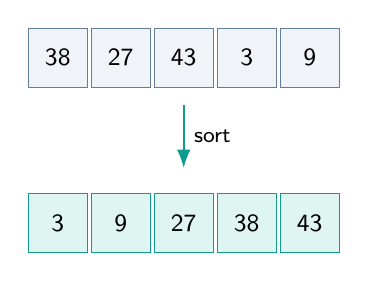
\begin{tikzpicture}[node distance=2mm,font=\small]
  \foreach \v/\x in {38/0,27/1,43/2,3/3,9/4}{
    \node[draw=grey,fill=lightgrey,minimum width=0.75cm,minimum height=0.75cm] at (\x*0.8,1.2) {\v};}
  \node at (2.4,1.2) {};
  \draw[-{Latex},teal,thick] (1.6,0.6) -- (1.6,-0.2) node[midway,right,black]{\footnotesize sort};
  \foreach \v/\x in {3/0,9/1,27/2,38/3,43/4}{
    \node[draw=teal,fill=tealLight,minimum width=0.75cm,minimum height=0.75cm] at (\x*0.8,-0.9) {\v};}
\end{tikzpicture}
\end{column}
\end{columns}
\end{frame}

% ============================================================
\begin{frame}{Overview of Three Algorithms}{At a glance}
\small
\begin{table}
\begin{tabular}{lccc}
\toprule
\textbf{Aspect} & \textbf{Merge Sort} & \textbf{Quick Sort} & \textbf{Heap Sort}\\
\midrule
Strategy & Divide \& Conquer & Divide \& Conquer & Selection via Heap\\
\rowcolor{lightgrey} Stable & Yes & No & No\\
In-place & No & Yes & Yes\\
\rowcolor{lightgrey} Worst case & \(\Theta(n\log n)\) & \(O(n^2)\) & \(O(n\log n)\)\\
Average case & \(\Theta(n\log n)\) & \(\Theta(n\log n)\) & \(\Theta(n\log n)\)\\
\rowcolor{lightgrey} Auxiliary space & \(O(n)\) & \(O(\log n)\) & \(O(1)\)\\
Key application & External sorting & General-purpose libs & Priority queues\\
\bottomrule
\end{tabular}
\end{table}
\end{frame}

\sectionsep{Merge Sort}

% ============================================================
\begin{frame}{Merge Sort --- Introduction \& History}
\begin{columns}[T]
\begin{column}{0.55\textwidth}
\begin{itemize}
  \item Comparison-based, \textbf{divide-and-conquer} algorithm
  \item Introduced by \textbf{John von Neumann}, 1945
  \item Splits array, sorts halves recursively, merges results
  \item Guarantees \(\Theta(n\log n)\) in \emph{all} cases
  \item \textbf{Stable} -- order of equal elements preserved
\end{itemize}
\end{column}
\begin{column}{0.45\textwidth}
\begin{block}{Motivation}
\small Simple sorts degrade to \(O(n^2)\) on large inputs. Merge Sort breaks the problem into smaller pieces solved independently, then combined -- a faster and more scalable strategy.
\end{block}
\end{column}
\end{columns}
\end{frame}

% ============================================================
\begin{frame}{Merge Sort --- Divide and Conquer}
\begin{center}
\begin{forest}
for tree={draw=teal,rounded corners,fill=tealLight,font=\scriptsize,l sep=6mm,s sep=3mm,edge={-{Latex},grey}}
[38\,27\,43\,3\,9\,82\,10
  [38\,27\,43
    [38\,27 [38] [27]]
    [43]]
  [3\,9\,82\,10
    [3\,9 [3] [9]]
    [82\,10 [82] [10]]]
]
\end{forest}
\end{center}
\vspace{2mm}
\begin{center}\small \(\log_2 n\) levels of splitting, each level costs \(\Theta(n)\) to merge back.\end{center}
\end{frame}

% ============================================================
\begin{frame}{Merge Sort --- Step-by-Step Execution}
\begin{overprint}
\onslide<1>\begin{center}\Large 38\;\;27\;\;43\;\;3\;\;9\;\;82\;\;10\\[4mm]\normalsize\color{grey} Initial unsorted array\end{center}
\onslide<2>\begin{center}\Large [38\;27\;43]\quad\quad[3\;9\;82\;10]\\[4mm]\normalsize\color{grey} Split into two halves\end{center}
\onslide<3>\begin{center}\Large [38][27\;43]\quad\quad[3\;9][82\;10]\\[4mm]\normalsize\color{grey} Split recursively until size 1}\end{center}
\onslide<4>\begin{center}\Large [27\;38\;43]\quad\quad[3\;9\;10\;82]\\[4mm]\normalsize\color{grey} Merge sorted sub-arrays}\end{center}
\onslide<5>\begin{center}\Large \color{teal}\bfseries 3\;\;9\;\;10\;\;27\;\;38\;\;43\;\;82\\[4mm]\normalsize\color{grey} Final merge -- fully sorted}\end{center}
\end{overprint}
\end{frame}

% ============================================================
\begin{frame}{Merge Sort --- Pseudocode}
\begin{algorithm}[H]
\footnotesize
\begin{algorithmic}[1]
\Procedure{MergeSort}{$A, left, right$}
  \If{$left < right$}
    \State $mid \gets \lfloor (left+right)/2 \rfloor$
    \State \Call{MergeSort}{$A, left, mid$}
    \State \Call{MergeSort}{$A, mid{+}1, right$}
    \State \Call{Merge}{$A, left, mid, right$}
  \EndIf
\EndProcedure
\Procedure{Merge}{$A, left, mid, right$}
  \State $L \gets A[left..mid]$, \quad $R \gets A[mid{+}1..right]$
  \State $i,j \gets 0,0$; \quad $k \gets left$
  \While{$i < |L|$ and $j < |R|$}
    \If{$L[i] \le R[j]$} $A[k]\gets L[i]$; $i{+}{+}$ \Else\ $A[k]\gets R[j]$; $j{+}{+}$ \EndIf
    \State $k \gets k+1$
  \EndWhile
  \State Copy remaining elements of $L$, $R$ into $A$
\EndProcedure
\end{algorithmic}
\end{algorithm}
\end{frame}

% ============================================================
\begin{frame}{Merge Sort --- Mathematical Foundation}
\begin{columns}[T]
\begin{column}{0.55\textwidth}
\[
T(n) = 2T\!\left(\frac{n}{2}\right) + \Theta(n), \quad T(1)=\Theta(1)
\]
Master Theorem: \(a=2,\ b=2,\ f(n)=\Theta(n)\)
\[
n^{\log_b a} = n^{\log_2 2} = n = f(n)
\]
\(\Rightarrow\) \textbf{Case 2} applies:
\[
\boxed{T(n) = \Theta(n\log n)}
\]
\end{column}
\begin{column}{0.45\textwidth}
\small Recursion-tree check: depth $k$ has $2^k$ subproblems of size $n/2^k$, each level costs $\Theta(n)$.
\[
\text{levels} = \log_2 n \;\Rightarrow\; \Theta(n)\times\log_2 n
\]
\end{column}
\end{columns}
\vspace{3mm}
\begin{table}\small
\begin{tabular}{lccc}
\toprule
Best & Average & Worst & Space\\
\midrule
\(\Omega(n\log n)\) & \(\Theta(n\log n)\) & \(O(n\log n)\) & \(O(n)\)\\
\bottomrule
\end{tabular}
\end{table}
\end{frame}

% ============================================================
\begin{frame}{Merge Sort --- Applications, Pros \& Cons}
\begin{columns}[T]
\begin{column}{0.5\textwidth}
\textbf{\color{teal}Advantages}
\begin{itemize}
  \item Guaranteed \(\Theta(n\log n)\), any input
  \item Stable -- preserves equal-key order
  \item Ideal for linked lists \& external sorting
\end{itemize}
\end{column}
\begin{column}{0.5\textwidth}
\textbf{\color{warnRed}Disadvantages}
\begin{itemize}
  \item Needs \(O(n)\) auxiliary space
  \item Not in-place
  \item Slower constant factor than Quick Sort
\end{itemize}
\end{column}
\end{columns}
\vspace{2mm}
\begin{block}{Applications}
\small External sorting on disk/tape, sorting linked lists, parallel/distributed sorting, and hybrid algorithms such as Timsort.
\end{block}
\end{frame}

\sectionsep{Quick Sort}

% ============================================================
\begin{frame}{Quick Sort --- Introduction \& History}
\begin{columns}[T]
\begin{column}{0.55\textwidth}
\begin{itemize}
  \item Invented by \textbf{Tony Hoare}, 1959 (published 1961)
  \item Divide-and-conquer via \textbf{pivot partitioning}
  \item Smaller elements left of pivot, larger to the right
  \item Sorts \textbf{in-place}; strong average-case speed
\end{itemize}
\end{column}
\begin{column}{0.45\textwidth}
\begin{block}{Motivation}
\small Merge Sort's \(\Theta(n)\) extra memory is costly at scale. Quick Sort needs only \(O(\log n)\) stack space, at the price of a quadratic worst case.
\end{block}
\end{column}
\end{columns}
\end{frame}

% ============================================================
\begin{frame}{Quick Sort --- Pivot \& Partition}
\begin{center}
\begin{tikzpicture}[font=\small]
  \foreach \v/\x in {9/0,4/1,8/2,3/3,1/4,2/5}{
    \node[draw=grey,fill=lightgrey,minimum width=0.8cm,minimum height=0.8cm] at (\x*0.85,1.4) {\v};}
  \node[draw=warnRed,thick] at (5*0.85,1.4) {2};
  \node[below=1mm of {(4.25,1.4)},font=\scriptsize,color=warnRed] {pivot};
  \draw[-{Latex},teal,thick] (2.1,0.8) -- (2.1,0.1);
  \foreach \v/\x/\c in {1/0,2/1,9/2,4/3,8/4,3/5}{
    \node[draw=\c,fill=tealLight,minimum width=0.8cm,minimum height=0.8cm] at (\x*0.85,-0.5) {\v};}
  \node[below=3mm of {(0.42,-0.5)},font=\scriptsize,color=teal]{\(\le\) pivot};
  \node[below=3mm of {(3.4,-0.5)},font=\scriptsize,color=warnRed]{\(>\) pivot};
\end{tikzpicture}
\end{center}
\vspace{2mm}
\begin{center}
\begin{forest}
for tree={draw=teal,rounded corners,fill=tealLight,font=\scriptsize,l sep=6mm,edge={-{Latex},grey}}
[9\,4\,8\,3\,1\,2
 [1\,2 [1] [2]]
 [9\,4\,8\,3]]
\end{forest}
\end{center}
\end{frame}

% ============================================================
\begin{frame}{Quick Sort --- Step-by-Step Execution}
\begin{overprint}
\onslide<1>\begin{center}\Large 9\;\;4\;\;8\;\;3\;\;1\;\;2\\[4mm]\normalsize\color{grey} Choose pivot = last element (2)\end{center}
\onslide<2>\begin{center}\Large [1\;2] \quad \textbf{2} \quad [9\;4\;8\;3]\\[4mm]\normalsize\color{grey} Partition around pivot\end{center}
\onslide<3>\begin{center}\Large [1] \; \textbf{2} \; [9\;4\;8\;3] \(\to\) recurse\\[4mm]\normalsize\color{grey} Recursively partition right side}\end{center}
\onslide<4>\begin{center}\Large [3][4][8][9]\\[4mm]\normalsize\color{grey} Sub-partitions resolve}\end{center}
\onslide<5>\begin{center}\Large\color{teal}\bfseries 1\;\;2\;\;3\;\;4\;\;8\;\;9\\[4mm]\normalsize\color{grey} Final sorted array}\end{center}
\end{overprint}
\end{frame}

% ============================================================
\begin{frame}{Quick Sort --- Pseudocode}
\begin{algorithm}[H]
\footnotesize
\begin{algorithmic}[1]
\Procedure{QuickSort}{$A, low, high$}
  \If{$low < high$}
    \State $p \gets$ \Call{Partition}{$A, low, high$}
    \State \Call{QuickSort}{$A, low, p-1$}
    \State \Call{QuickSort}{$A, p+1, high$}
  \EndIf
\EndProcedure
\Procedure{Partition}{$A, low, high$}
  \State $pivot \gets A[high]$; \quad $i \gets low-1$
  \For{$j \gets low$ \textbf{to} $high-1$}
    \If{$A[j] \le pivot$}
      \State $i \gets i+1$; \quad swap $A[i], A[j]$
    \EndIf
  \EndFor
  \State swap $A[i{+}1], A[high]$ \Return $i+1$
\EndProcedure
\end{algorithmic}
\end{algorithm}
\end{frame}

% ============================================================
\begin{frame}{Quick Sort --- Mathematical Foundation}
\[
T(n) = T(q) + T(n-1-q) + \Theta(n)
\]
\begin{columns}[T]
\begin{column}{0.33\textwidth}
\textbf{\color{warnRed}Worst} \(q=0\)
\[T(n)=T(n-1)+\Theta(n)\]
\[\Rightarrow \Theta(n^2)\]
\end{column}
\begin{column}{0.33\textwidth}
\textbf{\color{teal}Best} \(q\approx n/2\)
\[T(n)=2T(n/2)+\Theta(n)\]
\[\Rightarrow \Theta(n\log n)\]
\end{column}
\begin{column}{0.33\textwidth}
\textbf{Average} (expectation)
\[T(n)=\tfrac1n\sum_{q=0}^{n-1}\!\big(T(q)+T(n{-}1{-}q)\big)+\Theta(n)\]
\[\Rightarrow \Theta(n\log n)\]
\end{column}
\end{columns}
\vspace{3mm}
\small\color{grey} Solved via the substitution method -- randomization drives expected performance to the same class as Merge Sort.
\end{frame}

% ============================================================
\begin{frame}{Quick Sort --- Applications, Pros \& Cons}
\begin{columns}[T]
\begin{column}{0.5\textwidth}
\textbf{\color{teal}Advantages}
\begin{itemize}
  \item Fast average case, small constants
  \item In-place -- \(O(\log n)\) extra space
  \item Default choice in most libraries
\end{itemize}
\end{column}
\begin{column}{0.5\textwidth}
\textbf{\color{warnRed}Disadvantages}
\begin{itemize}
  \item \(O(n^2)\) worst case
  \item Not stable
  \item Sensitive to pivot choice
\end{itemize}
\end{column}
\end{columns}
\vspace{2mm}
\begin{block}{Applications}
\small General-purpose library sorts, in-memory sorting where auxiliary space is limited; basis for hybrids like Introsort.
\end{block}
\end{frame}

\sectionsep{Heap Sort}

% ============================================================
\begin{frame}{Heap Sort --- Introduction \& History}
\begin{columns}[T]
\begin{column}{0.55\textwidth}
\begin{itemize}
  \item Introduced by \textbf{J.\,W.\,J. Williams}, 1964
  \item Refined by \textbf{Robert W. Floyd}
  \item Treats array as a \textbf{binary heap}
  \item Repeatedly extracts max, places it in final position
  \item Worst case \(\Theta(n\log n)\), space \(O(1)\)
\end{itemize}
\end{column}
\begin{column}{0.45\textwidth}
\begin{block}{Motivation}
\small Combines Merge Sort's guaranteed bound with Quick Sort's in-place operation -- no trade-off needed between time and space.
\end{block}
\end{column}
\end{columns}
\end{frame}

% ============================================================
\begin{frame}{Heap Sort --- Binary Max-Heap}
\begin{columns}[T]
\begin{column}{0.55\textwidth}
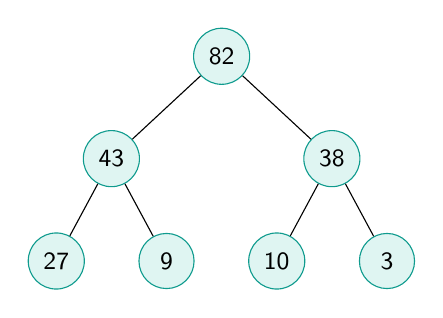
\begin{tikzpicture}[level distance=13mm,every node/.style={circle,draw=teal,fill=tealLight,minimum size=7mm,font=\small},
level 1/.style={sibling distance=28mm},level 2/.style={sibling distance=14mm}]
\node{82}
  child{node{43}
    child{node{27}}
    child{node{9}}}
  child{node{38}
    child{node{10}}
    child{node{3}}};
\end{tikzpicture}
\end{column}
\begin{column}{0.45\textwidth}
\small
Array form: \\[1mm]
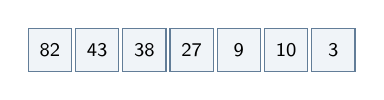
\begin{tikzpicture}[font=\scriptsize]
  \foreach \v/\x in {82/0,43/1,38/2,27/3,9/4,10/5,3/6}{
    \node[draw=grey,fill=lightgrey,minimum width=0.55cm,minimum height=0.55cm] at (\x*0.6,0) {\v};}
\end{tikzpicture}
\vspace{3mm}
\(\text{parent}(i) = \lfloor (i-1)/2 \rfloor\)\\[2mm]
Max-heap property: \(A[\text{parent}(i)] \ge A[i]\)\\[2mm]
Height: \(\lfloor \log_2 n \rfloor\)
\end{column}
\end{columns}
\end{frame}

% ============================================================
\begin{frame}{Heap Sort --- BuildHeap, Heapify, Extract-Max}
\begin{overprint}
\onslide<1>\begin{center}
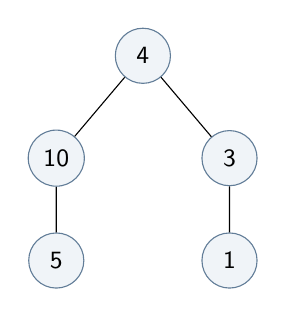
\begin{tikzpicture}[level distance=13mm,every node/.style={circle,draw=grey,fill=lightgrey,minimum size=7mm,font=\small},level 1/.style={sibling distance=22mm},level 2/.style={sibling distance=11mm}]
\node{4} child{node{10}child{node{5}}} child{node{3}child{node{1}}};
\end{tikzpicture}\\[2mm]\small\color{grey} Unsorted array as complete tree\end{center}
\onslide<2>\begin{center}
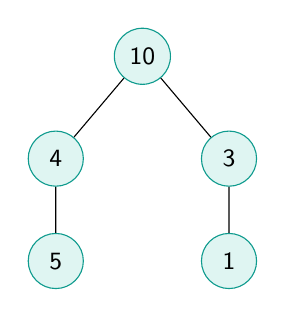
\begin{tikzpicture}[level distance=13mm,every node/.style={circle,draw=teal,fill=tealLight,minimum size=7mm,font=\small},level 1/.style={sibling distance=22mm},level 2/.style={sibling distance=11mm}]
\node{10} child{node{4}child{node{5}}} child{node{3}child{node{1}}};
\end{tikzpicture}\\[2mm]\small\color{grey} BuildMaxHeap -- Heapify bottom-up, \(O(n)\)\end{center}
\onslide<3>\begin{center}
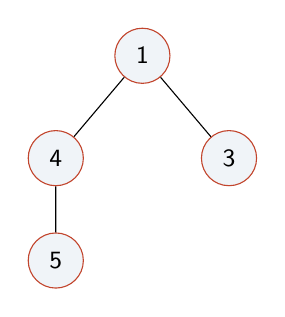
\begin{tikzpicture}[level distance=13mm,every node/.style={circle,draw=warnRed,fill=lightgrey,minimum size=7mm,font=\small},level 1/.style={sibling distance=22mm},level 2/.style={sibling distance=11mm}]
\node{1} child{node{4}child{node{5}}} child{node{3}};
\end{tikzpicture}\\[2mm]\small\color{grey} Extract max (10): swap with last, shrink heap\end{center}
\onslide<4>\begin{center}
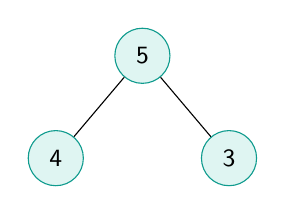
\begin{tikzpicture}[level distance=13mm,every node/.style={circle,draw=teal,fill=tealLight,minimum size=7mm,font=\small},level 1/.style={sibling distance=22mm}]
\node{5} child{node{4}} child{node{3}};
\end{tikzpicture}\\[2mm]\small\color{grey} Sift-down restores heap property, \(O(\log n)\)\end{center}
\onslide<5>\begin{center}\Large\color{teal}\bfseries 1\;\;3\;\;4\;\;5\;\;10\\[4mm]\normalsize\color{grey} Repeat extraction \(n{-}1\) times \(\to\) sorted array\end{center}
\end{overprint}
\end{frame}

% ============================================================
\begin{frame}{Heap Sort --- Pseudocode}
\begin{algorithm}[H]
\footnotesize
\begin{algorithmic}[1]
\Procedure{HeapSort}{$A$}
  \State $n \gets \text{length}(A)$; \quad \Call{BuildMaxHeap}{$A,n$}
  \For{$i \gets n-1$ \textbf{downto} $1$}
     \State swap $A[0], A[i]$; \quad \Call{MaxHeapify}{$A, 0, i$}
  \EndFor
\EndProcedure
\Procedure{MaxHeapify}{$A, i, heapSize$}
  \State $l\gets 2i{+}1$, $r\gets 2i{+}2$, $largest \gets i$
  \If{$l<heapSize$ and $A[l]>A[largest]$} $largest\gets l$ \EndIf
  \If{$r<heapSize$ and $A[r]>A[largest]$} $largest\gets r$ \EndIf
  \If{$largest \ne i$}
     \State swap $A[i], A[largest]$; \quad \Call{MaxHeapify}{$A, largest, heapSize$}
  \EndIf
\EndProcedure
\end{algorithmic}
\end{algorithm}
\end{frame}

% ============================================================
\begin{frame}{Heap Sort --- Complexity Derivation}
\begin{columns}[T]
\begin{column}{0.5\textwidth}
\textbf{Build-heap cost:}
\[
\sum_{h=0}^{\lfloor\log_2 n\rfloor}\left\lceil\frac{n}{2^{h+1}}\right\rceil O(h) = O\!\left(n\sum_{h=0}^{\infty}\frac{h}{2^h}\right)=O(n)
\]
using \(\sum h/2^h = 2\).
\end{column}
\begin{column}{0.5\textwidth}
\textbf{Overall cost:}
\[
T(n) = O(n) + \sum_{k=1}^{n-1}O(\log k) = \Theta(n\log n)
\]
\(n{-}1\) extract-max ops, each \(O(\log n)\) sift-down.
\end{column}
\end{columns}
\vspace{3mm}
\begin{table}\small
\begin{tabular}{lccc}
\toprule
Best & Average & Worst & Space\\
\midrule
\(\Omega(n\log n)\) & \(\Theta(n\log n)\) & \(O(n\log n)\) & \(O(1)\)\\
\bottomrule
\end{tabular}
\end{table}
\end{frame}

% ============================================================
\begin{frame}{Heap Sort --- Applications, Pros \& Cons}
\begin{columns}[T]
\begin{column}{0.5\textwidth}
\textbf{\color{teal}Advantages}
\begin{itemize}
  \item Guaranteed \(O(n\log n)\) worst case
  \item In-place, \(O(1)\) auxiliary space
  \item Asymptotically optimal comparison sort
\end{itemize}
\end{column}
\begin{column}{0.5\textwidth}
\textbf{\color{warnRed}Disadvantages}
\begin{itemize}
  \item Not stable
  \item Poor cache locality vs.\ Quick Sort
  \item Larger constant factor in practice
\end{itemize}
\end{column}
\end{columns}
\vspace{2mm}
\begin{block}{Applications}
\small Priority queues, real-time / embedded systems needing worst-case guarantees with minimal memory.
\end{block}
\end{frame}

\sectionsep{Mathematical Analysis}

% ============================================================
\begin{frame}{Recurrence Relations \& the Master Theorem}
\[
T(n) = aT\!\left(\frac{n}{b}\right) + f(n)
\]
\begin{table}\small
\begin{tabular}{lccc}
\toprule
& Merge Sort & Quick Sort (bal.) & Heap Sort (extract phase)\\
\midrule
\(a\) & 2 & 2 & 1 per level\\
\(b\) & 2 & 2 & --\\
\(f(n)\) & \(\Theta(n)\) & \(\Theta(n)\) & \(\Theta(\log n)\) per op\\
Case & 2 & 2 & direct sum\\
Result & \(\Theta(n\log n)\) & \(\Theta(n\log n)\) & \(\Theta(n\log n)\)\\
\bottomrule
\end{tabular}
\end{table}
\vspace{2mm}
\textbf{Asymptotic notations:}\quad
\(O(g)\): upper bound \quad \(\Omega(g)\): lower bound \quad \(\Theta(g)\): tight bound
\end{frame}

% ============================================================
\begin{frame}{Recursion Trees \& Complexity Growth}
\begin{columns}[T]
\begin{column}{0.5\textwidth}
\begin{forest}
for tree={draw=teal,fill=tealLight,rounded corners,font=\tiny,l sep=5mm,edge={-{Latex},grey}}
[$n$ [ $n/2$ [$n/4$][$n/4$]] [$n/2$ [$n/4$][$n/4$]]]
\end{forest}
\small\\ Depth \(\log_2 n\), \(\Theta(n)\) per level \(\Rightarrow \Theta(n\log n)\)
\end{column}
\begin{column}{0.5\textwidth}
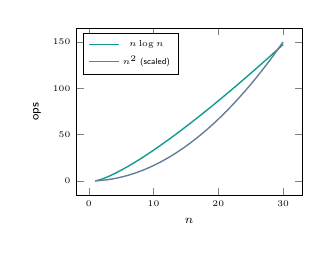
\begin{tikzpicture}[scale=0.62]
\begin{axis}[width=6.2cm,height=5cm,xlabel={$n$},ylabel={ops},legend pos=north west,
legend style={font=\tiny},label style={font=\scriptsize},tick label style={font=\tiny}]
\addplot[teal,thick,domain=1:30,samples=40]{x*ln(x)/ln(2)};
\addlegendentry{$n\log n$}
\addplot[grey,thick,domain=1:30,samples=40]{x^2/6};
\addlegendentry{$n^2$ (scaled)}
\end{axis}
\end{tikzpicture}
\end{column}
\end{columns}
\end{frame}

% ============================================================
\begin{frame}{Complexity Comparison}
\small
\begin{table}
\begin{tabular}{lccccccc}
\toprule
\textbf{Algo} & \textbf{Best} & \textbf{Avg} & \textbf{Worst} & \textbf{Space} & \textbf{Stable} & \textbf{In-place} & \textbf{Cache}\\
\midrule
Merge & \(\Omega(n\lg n)\) & \(\Theta(n\lg n)\) & \(O(n\lg n)\) & \(O(n)\) & Yes & No & Fair\\
\rowcolor{lightgrey} Quick & \(\Omega(n\lg n)\) & \(\Theta(n\lg n)\) & \(O(n^2)\) & \(O(\lg n)\) & No & Yes & Best\\
Heap & \(\Omega(n\lg n)\) & \(\Theta(n\lg n)\) & \(O(n\lg n)\) & \(O(1)\) & No & Yes & Weak\\
\bottomrule
\end{tabular}
\end{table}
\end{frame}

% ============================================================
\begin{frame}{When Should Each Algorithm Be Used?}
\begin{center}
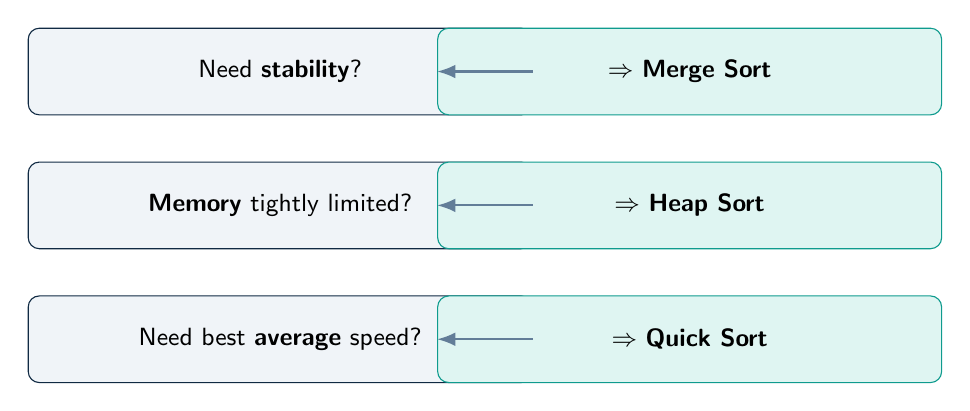
\begin{tikzpicture}[every node/.style={font=\small},box/.style={rectangle,rounded corners,draw=darkblue,fill=lightgrey,minimum width=6.4cm,minimum height=1.1cm,align=center}]
\node[box] (q1) at (0,3) {Need \textbf{stability}?};
\node[box,fill=tealLight,draw=teal] (m) at (5.2,3) {\(\Rightarrow\) \textbf{Merge Sort}};
\node[box] (q2) at (0,1.3) {\textbf{Memory} tightly limited?};
\node[box,fill=tealLight,draw=teal] (h) at (5.2,1.3) {\(\Rightarrow\) \textbf{Heap Sort}};
\node[box] (q3) at (0,-0.4) {Need best \textbf{average} speed?};
\node[box,fill=tealLight,draw=teal] (qs) at (5.2,-0.4) {\(\Rightarrow\) \textbf{Quick Sort}};
\draw[-{Latex},grey,thick] (q1) -- (m);
\draw[-{Latex},grey,thick] (q2) -- (h);
\draw[-{Latex},grey,thick] (q3) -- (qs);
\end{tikzpicture}
\end{center}
\end{frame}

% ============================================================
\begin{frame}{Key Takeaways}
\begin{itemize}
  \setlength\itemsep{5mm}
  \item Divide-and-conquer turns \(O(n^2)\) into \(\Theta(n\log n)\)
  \item Merge Sort: stable, reliable, needs extra space
  \item Quick Sort: fast in practice, in-place, risky worst case
  \item Heap Sort: optimal worst case, in-place, weaker cache use
\end{itemize}
\end{frame}

% ============================================================
\begin{frame}{Conclusion}
\begin{itemize}
  \item All three achieve \(\Theta(n\log n)\) on average -- the optimal bound for comparison sorts
  \item Choice depends on \textbf{stability}, \textbf{memory}, and \textbf{data} characteristics
  \item Recurrences, the Master Theorem, and recursion trees give rigorous proof of performance
  \item Real systems often blend these ideas -- \emph{Timsort}, \emph{Introsort}
\end{itemize}
\end{frame}

% ============================================================
\begin{frame}[plain]
\begin{tikzpicture}[remember picture,overlay]
  \fill[darkblue] (current page.south west) rectangle (current page.north east);
  \fill[teal] (current page.south west) rectangle ++(\paperwidth,0.6);
  \node[white,align=center] at (current page.center) {
    \begin{minipage}{0.8\paperwidth}
      \centering
      {\Huge\bfseries Questions?}\\[8mm]
      {\Large Thank You}\\[4mm]
      {\small Group 7 \(\cdot\) DSMA-123: Data Structures \(\cdot\) Kathmandu University}
    \end{minipage}
  };
\end{tikzpicture}
\end{frame}

% ============================================================
\begin{frame}{References}
\footnotesize
\begin{enumerate}
  \item T.\,H. Cormen, C.\,E. Leiserson, R.\,L. Rivest, C. Stein, \textit{Introduction to Algorithms}, 3rd ed., MIT Press, 2009.
  \item D.\,E. Knuth, \textit{The Art of Computer Programming, Vol.\,3: Sorting and Searching}, 2nd ed., Addison-Wesley, 1998.
  \item M.\,T. Goodrich, R. Tamassia, M.\,H. Goldwasser, \textit{Data Structures and Algorithms in Python}, Wiley, 2013.
  \item S.\,S. Skiena, \textit{The Algorithm Design Manual}, 2nd ed., Springer, 2008.
\end{enumerate}
\end{frame}

\end{document}